\chapter{The Latent Cognition Trilogy} \footnotemark{}
%=====================================
% Leocadio, Paulo, A Transformer-Based Framework % for 
% Automated Incident Response in Cybersecurity 
% (March 19, 2026). 
% Full original paper available at SSRN: 
% https://ssrn.com/abstract=6821299 
% or %http://dx.doi.org/10.2139/ssrn.6821299
%=====================================
% \begin{longtable}[]{@{}
% >{\raggedright\arraybackslash}p{(\columnwidth - 6\tabcolsep) * \real{0.0727}}
% >{\raggedright\arraybackslash}p{(\columnwidth - 6\tabcolsep) * \real{0.3570}}
%  >{\raggedright\arraybackslash}p{(\columnwidth - 6\tabcolsep) * \real{0.0727}}
%  >{\raggedright\arraybackslash}p{(\columnwidth - 6\tabcolsep) * \real{0.4975}}@{}}
% \caption{}
% \tabularnewline
% \toprule()
% \begin{minipage}[b]{\linewidth}\raggedright
% 
\includegraphics[width=0.3in, height=0.3in] {figures/prologue_a.png}
% \end{minipage} & \begin{minipage}[b]{\linewidth}\raggedright
% 0000-0002-4992-4541
% \end{minipage} & \begin{minipage}[b]{\linewidth}\raggedright
% 
\includegraphics[width=0.31304in, height=0.3in] {figures/prologue_b.png}
% \end{minipage} & \begin{minipage}[b]{\linewidth}\raggedright
% 10.2139/ssrn.6821299
% \end{minipage} 
% \endfirsthe% ad
% \toprule% ()
% \begin{minipage}[b]{\linewidth}\raggedright
% 
\includegraphics[width=0.3in, height=0.3in] {figures/prologue_b.png}
% \end{minipage} & \begin{minipage}[b]{\linewidth}\raggedright
% 0000-0002-4992-4541
% \end{minipage} & \begin{minipage}[b]{\linewidth}\raggedright
%
\includegraphics[width=0.31304in, height=0.3in]{figures/prologue_b.png}
% \end{minipage} & \begin{minipage}[b]{\linewidth}\raggedright
% 10.2139/ssrn.6821299
% \end{minip% age} \\
% \midrule% ()
% \endhe% ad
% \bottomrule()
% \end{longtable% }

\section{Contextual overview} 
\footnotetext{Chapter originally released under DOI 10.2139/ssrn.6821299 by ORCID:0000-0002-4992-4541}.

The problem addressed in this work is the persistent separation between parametric memory, encoded within model weights, and non-parametric memory retrieved through external databases or retrieval systems in modern \textbf{Retrieval-Augmented Generation} (\textbf{RAG}) architectures. Although RAG-based systems have improved factual grounding in \textbf{large language models} (\textbf{LLMs}), they introduce architectural fragmentation between the retrieval and generation components, which are often optimized independently and coupled only at inference time.

This separation introduces several limitations, including retrieval latency, semantic drift between the retrieved evidence and the model's context, and restricted end-to-end gradient flow between evidence selection and downstream reasoning. Existing memory-augmented architectures partially address these issues but typically maintain retrieval as an external or weakly integrated process.

The \emph{DLI-LLM framework} proposes an alternative architectural formulation in which differentiable retrieval mechanisms are integrated directly into Transformer layers via a latent key-value memory structure \cite{Bahdanau2015}. Retrieval queries are generated from hidden-state representations and routed through learned attention-gating mechanisms, enabling the retrieved vectors to participate directly within the transformer\textquotesingle s forward computation pathway.

The objective of this paper is not to claim empirical validation but to formalize the architectural implications, theoretical properties, and comparative positioning of a retrieval-integrated transformer architecture within the broader landscape of retrieval- and memory-augmented transformer architectures \cite{Lewis2021, Khandelwal2020, Qu2021, Schmid2011}.

\hypertarget{introduction}{%
\section{Introduction}
\label{introduction}}

Retrieval-Augmented Generation (RAG) architectures have improved factual grounding in large language models (LLMs) by combining parametric generation with external retrieval systems. However, these architectures often maintain an operational separation between retrieval and inference, leading to architectural fragmentation, increased retrieval latency, and limited end-to-end differentiability between evidence selection and downstream generation.

This separation introduces several limitations, including retrieval latency, semantic drift between the retrieved evidence and the model's context, and restricted end-to-end gradient flow between evidence selection and downstream reasoning. Existing memory-augmented architectures partially address these issues but typically maintain retrieval as an external or weakly integrated process.

\emph{The DLI-LLM framework proposes an alternative architecture in which differentiable retrieval mechanisms are integrated directly into Transformer layers via a latent key-value memory structure.} Retrieval queries are generated from hidden-state representations and routed through learned attention-gating mechanisms, enabling the retrieved vectors to participate directly in the forward computation.

The objective of this paper is not to claim empirical validation, but to formalize the architectural implications, theoretical properties, and comparative positioning of this retrieval-integrated transformer architecture framework within the broader landscape of retrieval-augmented and memory-augmented transformer architectures.

\hypertarget{contributions}{%
\subsection{Contributions}}
\label{contributions}

This work contributes:

\begin{itemize}
\item  A conceptual architectural framework that integrates latent memory retrieval directly into transformer computation pathways.
\item  A mathematically formulated retrieval mechanism with differentiable routing and integration of latent key-value memory.
\item  A theoretical blueprint for retrieval-integrated transformer architectures operating within the forward computation graph.
\item  A comparative analysis situating DLI-LLM relative to retrieval-augmented and memory-augmented transformer systems.
\item  A structured discussion of theoretical behaviors, architectural limitations, and future experimental directions associated with differentiable latent retrieval.
\end{itemize}

\hypertarget{overview-of-the-paper}{%
\subsection{Overview of the Paper}}
\label{overview-of-the-paper}

\textbf{Section 2} develops the methodological and \emph{architectural foundation of the DLI-LLM framework}\footnotemark{} by decomposing the originating hypothesis into its principal architectural components. The section formalizes the retrieval mechanism through mathematical definitions, algorithmic specification, and implementation-oriented architectural modeling. It also situates the proposed framework in relation to existing retrieval- and memory-augmented transformer architectures through comparative analysis.
\footnotetext{This chapter is available on SSRN at 6821299 or via DOI 10.2139/ssrn.6821299}. Originally written as a journal paper, this piece was later included in the book as a prologue because it describes the architectural phenomenon that inspired the broader investigation.

\textbf{Section 3} examines the predicted architectural behaviors and limitations of differentiable latent retrieval, including retrieval dynamics, memory-scaling considerations, retrieval coherence, and potential failure modes, in the absence of an empirical implementation.
\textbf{Section 4} discusses broader implications for the design of retrieval-integrated transformer architectures, internal memory architectures, and future experimental investigations.
\hypertarget{architectural-framework-and-methodology}{%
\section{Architectural Framework and Methodology}}
\label{architectural-framework-and-methodology}
This paper does not present empirical validation or benchmarked implementation results. Instead, it develops a conceptual architectural framework based on the \textbf{Differentiable Latent} \textbf{Indexing} inside \emph{Large Language Models (DLI-LLM) hypothesis}, as reproduced in \textbf{Appendix A}. The methodology follows a structured process of architectural decomposition, mathematical formalization, comparative analysis, and implementation-oriented modeling to examine how differentiable retrieval mechanisms can be integrated directly into transformer computational pathways.
\hypertarget{architectural-foundations}{%
\subsection{Architectural Foundations}}
\label{architectural-foundations}
The \emph{DLI-LLM framework} is derived from four principal architectural assumptions:
\begin{enumerate}
\item The integration of a differentiable memory module within transformer layers.
\item The use of latent key-value memory structures to support scalable retrieval operations.
\item The existence of a shared latent vector space for token representations and retrieved document embeddings.
\item A learned routing-and-gating mechanism that dynamically controls retrieval activation during inference.
\end{enumerate}
Together, these components define a retrieval-integrated transformer architecture in which latent memory access is integrated into the forward computation rather than occurring as an external retrieval stage.
Unlike conventional \textbf{Retrieval-Augmented Generation} (\textbf{RAG}) systems, in which retrieval and generation are often decoupled, DLI-LLM embeds retrieval directly into transformer-layer operations. Retrieval queries are generated from hidden-state representations and used to access latent memory structures through differentiable similarity functions. Retrieved vectors are subsequently fused back into the attention pathway through learned gating mechanisms.
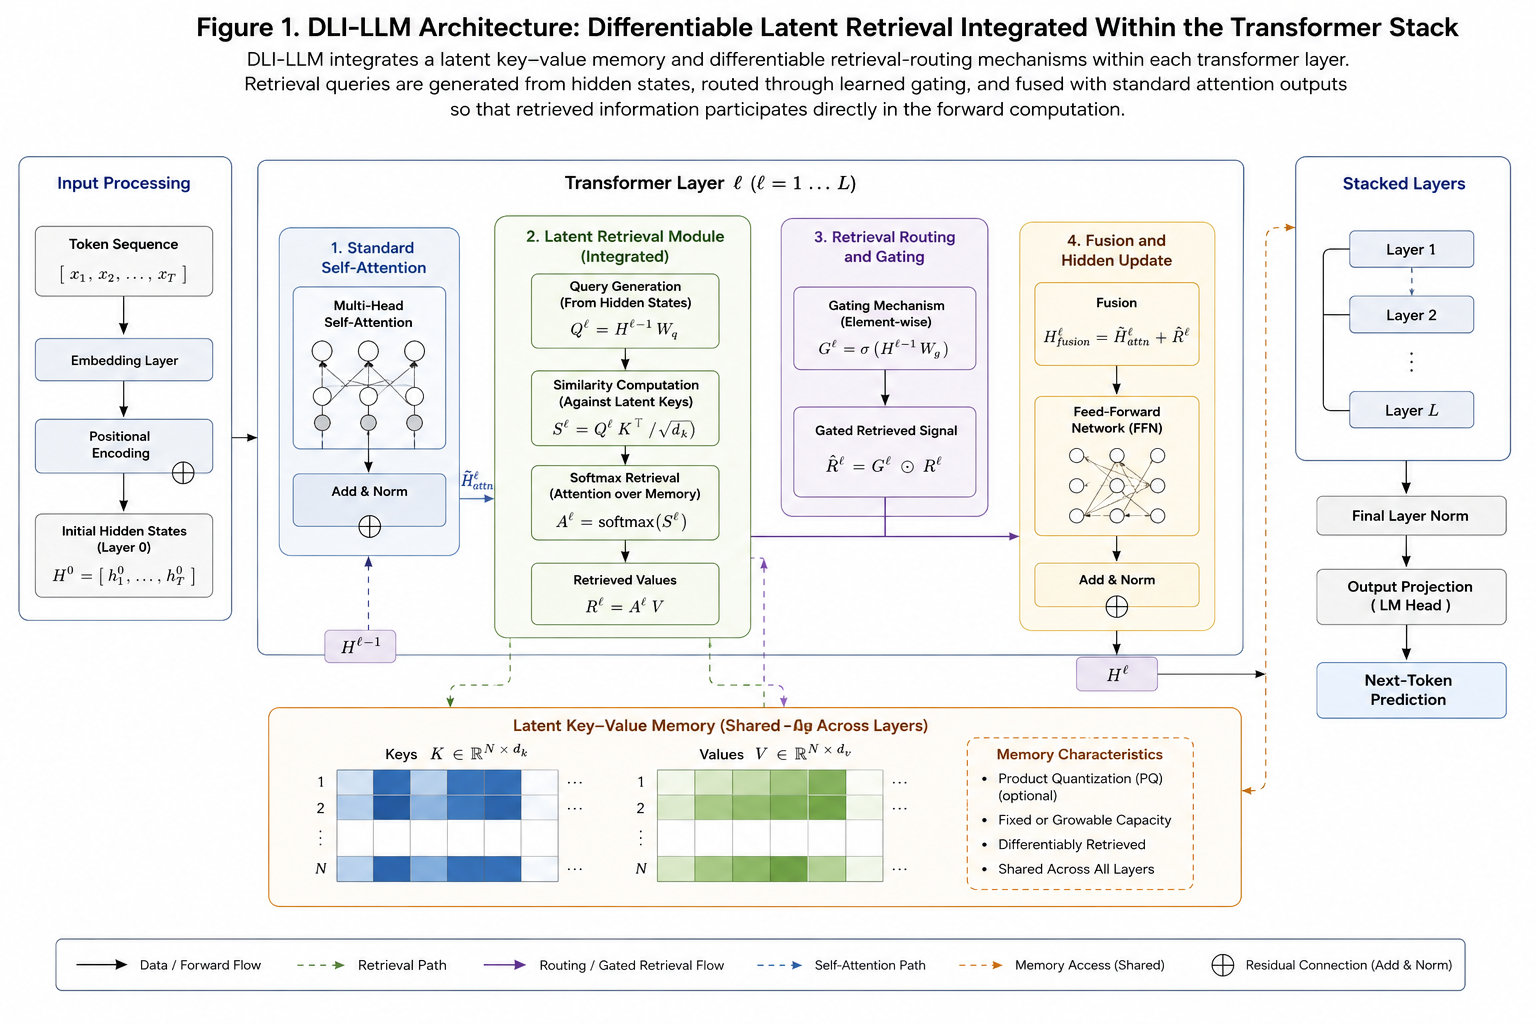
\includegraphics[width=5in,height=3.33333in]{figures/prologue1.png}
\textbf{Figure 1} illustrates the conceptual retrieval pathway and latent memory integration process within the transformer stack.
\hypertarget{latent-memory-representation}{%
\subsection{Latent Memory Representation}}
\label{latent-memory-representation}
The proposed framework assumes the existence of a latent key-value memory structure:
\[M = \{(k_{i},v_{i})\}_{i = 1}^{N},k_{i},v_{i} \in \mathbb{R}^{d}
\]
The architecture assumes that both token representations and retrieved document embeddings can coexist in a shared latent vector space, enabling retrieval operations to occur in the same representational domain as transformer hidden states.
To support scalability, the framework optionally incorporates product quantization strategies inspired by large-scale vector retrieval systems and differentiable memory architectures. This enables latent retrieval to remain computationally tractable even when memory capacity grows substantially.
\hypertarget{retrieval-and-routing-mechanism}{%
\subsection{Retrieval and Routing Mechanism}}
\label{retrieval-and-routing-mechanism}
At each transformer layer, the hidden representation:
\[h_{t} \in \mathbb{R}^{d}
\]
\[q_{t} = W_{q}h_{t}
\]
\[s_{i} = \langle q_{t},k_{i}\rangle
\]
\[\alpha_{i} = \frac{\exp(s_{i}/\tau)}{\sum_{j}^{}{\exp(}s_{j}/\tau)}\]
where \(\tau\) denotes a temperature parameter that controls the sharpness of retrieval.
The retrieved latent representation becomes:
\[r_{t} = \sum_{i = 1}^{N}\alpha_{i}v_{i}\]
A learned routing gate modulates integration between retrieved memory and the original transformer hidden state:
\[g_{t} = \sigma(W_{g}\lbrack h_{t};r_{t}\rbrack)\]
The fused representation is subsequently computed as:
\[{\widetilde{h}}_{t} = g_{t} \cdot r_{t} + (1 - g_{t}) \cdot h_{t}\]

This formulation enables retrieved latent memory vectors to participate directly in transformer-layer computation \cite{Vaswani2017} while preserving differentiable gradient propagation through both the retrieval and attention pathways \cite{Graves2014,Graves2016,Santoro2016}

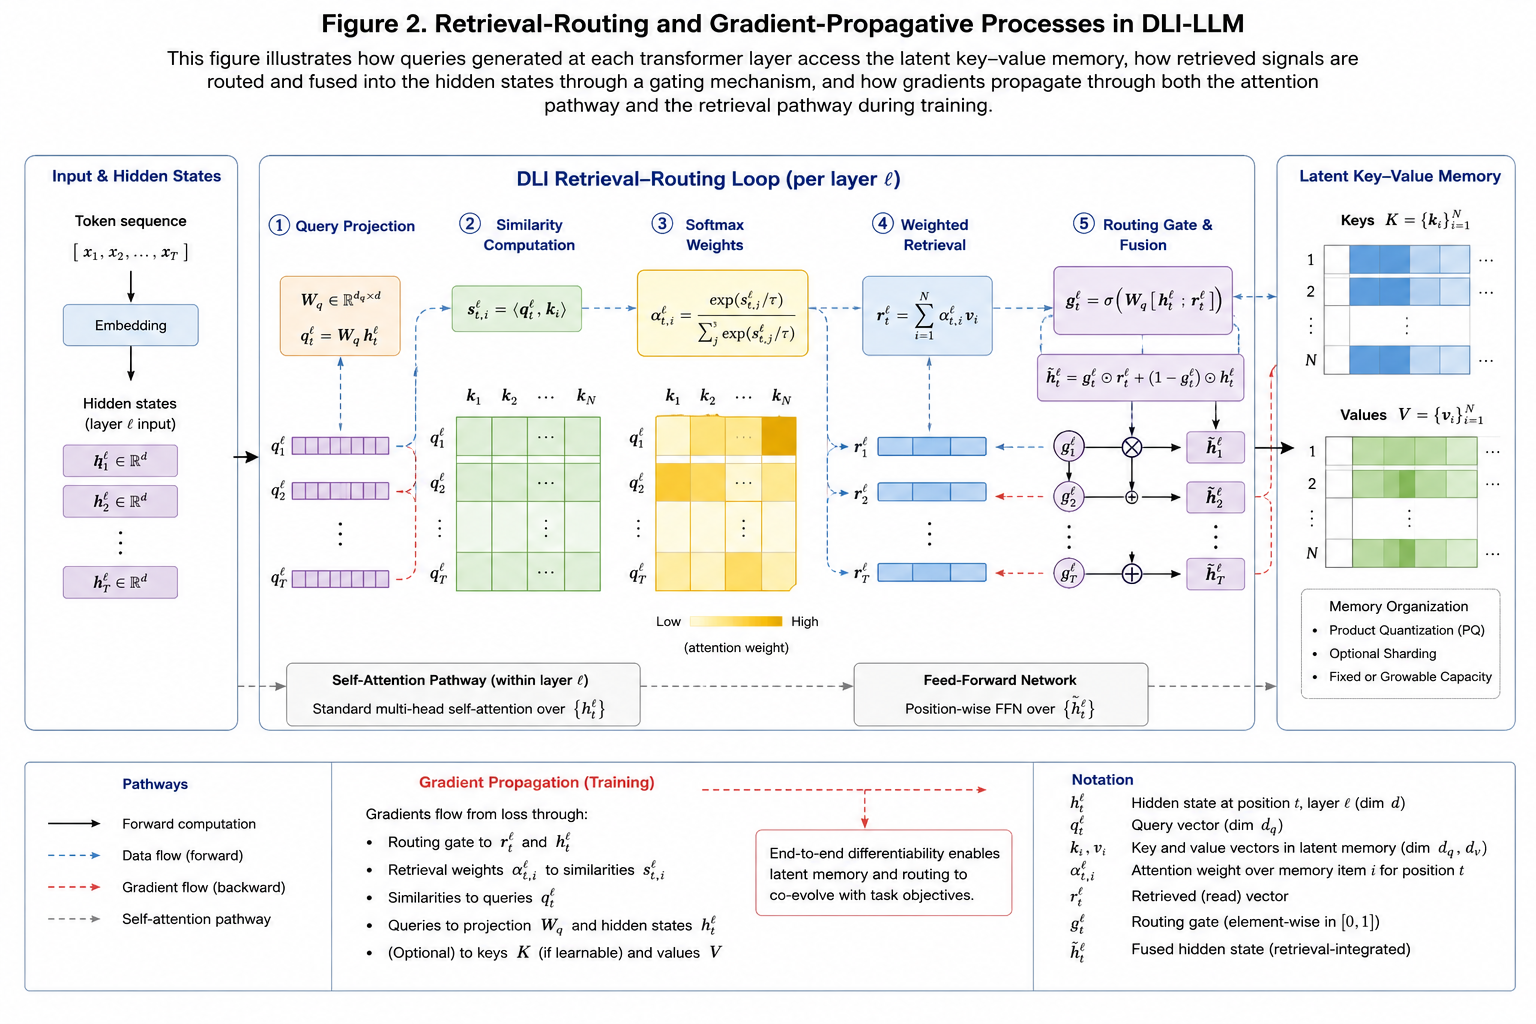
\includegraphics[width=5.5in,height=3.66667in]{figures/prologue2.png}

\textbf{Figure} 2 illustrates the retrieval-routing and gradient-propagation processes within the proposed framework.

\hypertarget{mathematical-interpretation}{%
\subsection{Mathematical Interpretation}}
\label{mathematical-interpretation}
The proposed formulation extends the standard transformer computation by introducing a differentiable retrieval pathway that operates alongside self-attention mechanisms. Unlike external retrieval architectures, in which retrieval systems operate independently of the language model, DLI-LLM integrates retrieval directly into the computational graph.
The framework draws conceptually on differentiable memory systems, attention-based addressing mechanisms, neural memory architectures, and retrieval-augmented transformer systems \cite{Graves2016}. However, the distinguishing feature of DLI-LLM is the integration of latent retrieval directly within transformer-layer computation rather than through externally orchestrated retrieval pipelines.
The resulting architecture enables retrieval decisions, routing behavior, and memory integration to evolve jointly during optimization through shared gradient propagation.
\hypertarget{algorithmic-retrieval-process}{%
\subsection{Algorithmic Retrieval Process}}
\label{algorithmic-retrieval-process}
\textbf{Algorithm 1} summarizes a single retrieval operation within one transformer layer.
\textbf{Input:} Hidden state \(h_{t}\), latent memory
\(M = \{(k_{i},v_{i})\}\), parameters \(W_{q},W_{g}\)
\textbf{Algorithm 1:} Differentiable Latent Retrieval Step
\textbf{Output:} Fused representation \({\widetilde{h}}_{t}\)

\begin{enumerate}
\def\labelenumi{\Alph{enumi}.}
\item \(q_{t} \leftarrow W_{q}h_{t}\)
\item Compute similarity scores \(s_{i} = \langle q_{t},k_{i}\rangle\)
\item Compute retrieval weights \(\alpha = \text{softmax}(s/\tau)\)
\item Retrieve latent vector:
\end{enumerate}

\[r_{t} = \sum_{i}^{}\alpha_{i}v_{i}\]

\begin{enumerate}
\def\labelenumi{\Alph{enumi}.}
\setcounter{enumi}{4}
\item Compute routing gate:
\end{enumerate}

\[g_{t} = \sigma(W_{g}\lbrack h_{t};r_{t}\rbrack)\]
\begin{enumerate}
\def\labelenumi{\Alph{enumi}.}
\setcounter{enumi}{5}
\tightlist
\item
\end{enumerate}
\[{\widetilde{h}}_{t} = g_{t} \cdot r_{t} + (1 - g_{t}) \cdot h_{t}\]
\begin{enumerate}
\def\labelenumi{\Alph{enumi}.}
\setcounter{enumi}{6}
\item  Return \({\widetilde{h}}_{t}\)
\end{enumerate}

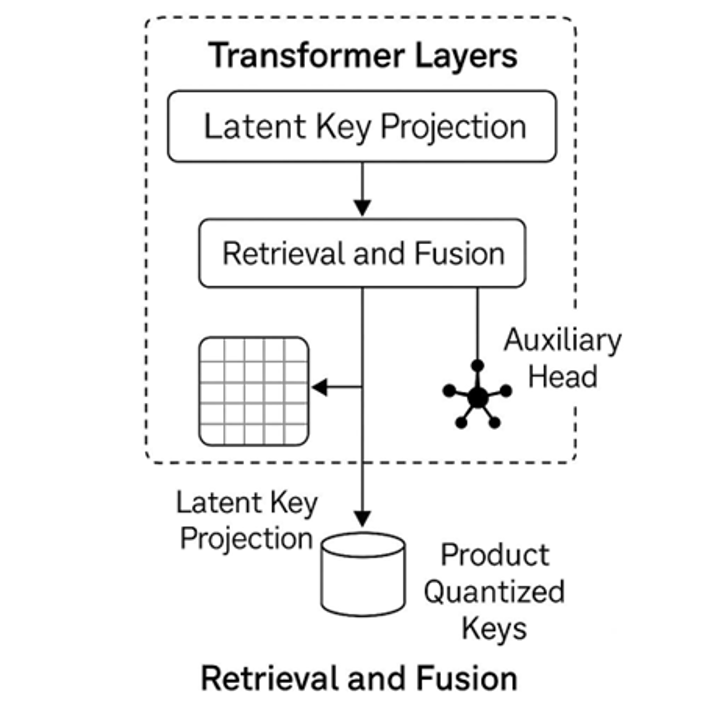
\includegraphics[width=4.83403in,height=4.83403in]{figures/prologue3.png}

\textbf{Figure} 3 presents the conceptual computational graph for the retrieval-routing process.
\hypertarget{conceptual-implementation-framework}{%
\subsection{Conceptual Implementation Framework}}
\label{conceptual-implementation-framework}
Although this work remains theoretical, an implementation-oriented DLI prototype would conceptually involve four principal stages:
\textbf{Memory Construction}

\begin{itemize}
\item  Extraction of latent document embeddings
\item  Construction of latent key-value memory banks
\item  Optional application of product quantization strategies for scalable retrieval
\end{itemize}

\textbf{Transformer Layer Integration}

\begin{itemize}
\item  Insertion of DLI retrieval blocks after self-attention layers
\item  Integration of learned routing and gating mechanisms
\item  Fusion of retrieved latent vectors within the transformer layer computation
\end{itemize}

\textbf{Training Objective}
A conceptual joint objective may combine language modeling and retrieval optimization:
\[\mathcal{L =}\mathcal{L}_{LM} + \lambda\mathcal{L}_{retrieval}\]
where \(\lambda\) controls the relative contribution of retrieval optimization.
\textbf{Inference Behavior}
Potential inference configurations may include:

\begin{itemize}
\item  Frozen latent memory
\item  Sparse top-k retrieval
\item  Memory sharding
\item  External memory swapping mechanisms
\end{itemize}

\hypertarget{comparative-architecture-analysis}{%
\subsection{Comparative Architecture Analysis}}
\label{comparative-architecture-analysis}

The \emph{DLI-LLM framework} conceptually intersects with multiple memory-augmented and retrieval-integrated transformer architectures \cite{Wu2022}.

\begin{longtable}[]{@{}
  >{\raggedright\arraybackslash}p{(\columnwidth - 4\tabcolsep) * \real{0.2849}}
  >{\raggedright\arraybackslash}p{(\columnwidth - 4\tabcolsep) * \real{0.3257}}
  >{\raggedright\arraybackslash}p{(\columnwidth - 4\tabcolsep) * \real{0.3894}}@{}}

\toprule()
\begin{minipage}[b]{\linewidth}\raggedright
\textbf{Architecture}
\end{minipage} & \begin{minipage}[b]{\linewidth}\raggedright
\textbf{Relation to DLI-LLM}
\end{minipage} & \begin{minipage}[b]{\linewidth}\raggedright
\textbf{Limitation Relative to DLI-LLM}
\end{minipage} \\
\midrule()

\endhead

Transformer-XL & Long-context recurrence & No latent key-value retrieval \\
RETRO & External retrieval augmentation & Retrieval remains externally orchestrated \\
Memorizing Transformers & Learnable memory tokens & No unified latent retrieval pathway \\
Differentiable Neural Computers & Key-value differentiable memory & Not integrated into transformer-layer computation \\
Recurrent Memory Transformers & Persistent memory states & Limited retrieval routing flexibility \\
KNN-LM & Post-hoc retrieval augmentation & Retrieval remains external and non-differentiable \\
Perceiver IO & Latent bottleneck architecture & No integrated latent retrieval routing \\
Hyena Hierarchy & Long-range implicit sequence modeling & No explicit memory retrieval mechanism \\
\bottomrule()
\end{longtable}

\hypertarget{limitations-and-theoretical-scope}{%
\subsection{Limitations and Theoretical Scope}}
\label{limitations-and-theoretical-scope}

This work does not present empirical implementation, benchmark evaluation, or experimental validation. The proposed framework should therefore be interpreted as a conceptual architectural model for formalizing differentiable latent retrieval within transformer-based systems.
Several limitations remain unresolved, including:

\begin{itemize}
\item  computational scaling of latent memory structures,
\item  memory saturation and retrieval interference,
\item  retrieval interpretability,
\item  training stability,
\item and the computational overhead associated with differentiable memory routing.
\end{itemize}

The framework also assumes that it is feasible to jointly optimize retrieval and language modeling objectives within a unified transformer computation graph, an assumption that requires future empirical validation.
Accordingly, the present work should be understood as a theoretical systems architecture proposal designed to motivate future implementation-oriented and experimental investigations into retrieval-integrated transformer architectures.

\hypertarget{predicted-architectural-behaviors}{%
\section{Predicted Architectural Behaviors}}
\label{predicted-architectural-behaviors}

Because this work does not present empirical implementation or benchmark evaluation, the behaviors discussed in this section should be interpreted as theoretical architectural predictions derived from the proposed \emph{DLI-LLM framework} and related findings in prior memory-augmented language model research.

\hypertarget{predicted-retrieval-and-memory-behaviors}{%
\subsection{Predicted Retrieval and Memory Behaviors}}
\label{predicted-retrieval-and-memory-behaviors}

\hypertarget{retrieval-efficiency}{%  
\subsubsection{Retrieval Efficiency}}
\label{retrieval-efficiency}

By integrating retrieval directly into the transformer's forward pass, DLI-LLM may reduce the external retrieval bottlenecks commonly associated with Retrieval-Augmented Generation (RAG) architectures \cite{Wu2022}. This prediction is consistent with prior observations that reducing external retrieval overhead can improve retrieval efficiency and inference coordination in memory-augmented systems.
\hypertarget{grounding-stability-and-hallucination-reduction}{%
\subsubsection{Grounding Stability and Hallucination Reduction}}
\label{grounding-stability-and-hallucination-reduction}
The integration of latent memory retrieval pathways may improve contextual grounding during generation by enabling retrieved latent representations to participate directly in transformer-layer computation. Similar retrieval-assisted grounding effects have been observed in retrieval-augmented generators and nearest-neighbor language models.
\hypertarget{memory-assisted-generalization}{%
\subsubsection{Memory-Assisted Generalization}
\label{memory-assisted-generalization}}
Because latent memory retrieval is integrated differentiably within transformer layers, the framework may exhibit memory-assisted generalization similar to that observed in hybrid retrieval and memory-augmented architectures.
\hypertarget{few-shot-adaptation-dynamics}{%
\subsubsection{Few-Shot Adaptation Dynamics}}
\label{few-shot-adaptation-dynamics}
The proposed routing and gating mechanisms may improve adaptation under limited supervision by selectively integrating retrieved latent representations according to contextual relevance. Similar dynamics have been reported in memory-augmented neural systems employing differentiable memory access.
\hypertarget{long-context-retrieval-coherence}{%
\subsubsection{Long-Context Retrieval Coherence}}
\label{long-context-retrieval-coherence}
Cross-layer retrieval propagation may improve retrieval consistency across extended token sequences by allowing latent memory interactions to evolve throughout transformer-layer computation. This behavior aligns conceptually with trends observed in long-context and persistent-memory transformer architectures \cite{Bulatov2022}.
\hypertarget{predicted-failure-modes-and-architectural-risks}{%
\subsection{Predicted Failure Modes and Architectural Risks}}
\label{predicted-failure-modes-and-architectural-risks}
\hypertarget{memory-saturation}{%\subsubsection{Memory Saturation}
\label{memory-saturation}}
As with other memory-augmented architectures, finite latent memory capacity may lead to retrieval saturation under large-scale document loads or prolonged retrieval accumulation.
\hypertarget{retrieval-redundancy}{%
\subsubsection{Retrieval Redundancy}}
\label{retrieval-redundancy}
High-dimensional latent retrieval may yield semantically redundant value-vector patterns, potentially reducing retrieval precision without appropriate compression or quantization.
\hypertarget{contextual-retrieval-drift}{%
\subsubsection{Contextual Retrieval Drift}}
\label{contextual-retrieval-drift}
Cross-layer retrieval propagation may introduce retrieval-context misalignment when latent query representations diverge from earlier contextual states. Similar forms of retrieval instability have been observed in persistent memory architectures.
\hypertarget{retrieval-poisoning-and-memory-contamination}{%
\subsubsection{Retrieval Poisoning and Memory Contamination}}
\label{retrieval-poisoning-and-memory-contamination}
Because latent retrieval pathways participate directly in transformer computation, corrupted or adversarial memory representations may propagate erroneous retrieval signals throughout downstream generation pathways. This introduces potential risks associated with latent memory contamination and retrieval integrity.
\hypertarget{comparative-architectural-behavior-analysis}{%
\subsection Comparative Architectural Behavior Analysis}
\label{comparative-architectural-behavior-analysis}
\hypertarget{discussion}{%
\section{Discussion}}
\label{discussion}
The \emph{DLI-LLM framework} proposes a retrieval-integrated transformer architecture in which latent memory access is incorporated into the forward-computation pathway rather than into an externally orchestrated retrieval stage. This architectural formulation has implications for how memory coordination, retrieval dynamics, and contextual grounding may be modeled within transformer-based systems.
\hypertarget{retrieval-integration-and-memory-coordination}{%
\subsection{Retrieval Integration and Memory Coordination}}
\label{retrieval-integration-and-memory-coordination}
By embedding differentiable latent retrieval directly within transformer layers, the proposed framework reduces the operational separation between retrieval and inference commonly observed in Retrieval-Augmented Generation (RAG) architectures. Similar principles have appeared in memory-augmented neural systems and differentiable memory architectures. However, DLI-LLM extends these concepts by integrating shared latent retrieval pathways that operate directly within transformer-layer computation.
The proposed framework suggests that retrieved latent representations may participate directly in contextual computation rather than functioning as externally injected retrieval artifacts.
\hypertarget{learning-dynamics-and-adaptation}{%
\subsection{Learning Dynamics and Adaptation}}
\label{learning-dynamics-and-adaptation}
The framework also suggests potential implications for continual learning and adaptive memory integration \cite{irwin2026mlf}because latent memory structures can be updated independently of full model retraining, and retrieval-integrated transformer architectures could support incremental memory adaptation amid evolving information conditions.
At the same time, this flexibility introduces architectural challenges associated with memory scaling, retrieval interference, latent redundancy, and retrieval saturation. Efficient pruning, quantization, and routing strategies will likely be necessary to maintain stable
retrieval behavior at scale.
\hypertarget{bias-safety-and-retrieval-integrity}{%
\subsection{Bias, Safety, and Retrieval Integrity}}
\label{bias-safety-and-retrieval-integrity}
Integrating retrieval pathways directly within transformer computation also introduces safety and interpretability considerations. Latent memory structures may preserve biased, corrupted, or privacy-sensitive representations that become difficult to inspect once integrated into
differentiable retrieval pathways.
These concerns partially resemble challenges observed in
retrieval-augmented systems. Still, they may become more difficult to isolate when retrieval coordination occurs internally through latent routing mechanisms rather than through externally inspectable retrieval pipelines.
\hypertarget{routing-and-architectural-control}{%
\subsection{Routing and Architectural Control}}
\label{routing-and-architectural-control}
A central component of the proposed framework is the retrieval-routing gate, which regulates how retrieved latent vectors influence transformer hidden states. This routing process determines the degree to which retrieved memory participates in downstream computation and contextual inference.
\textbf{Figure 4} presents a conceptual comparison between DLI-LLM and conventional retrieval-augmented architectures across multiple architectural dimensions, including retrieval coordination, grounding stability, memory coherence, and the distribution of retrieval failures.
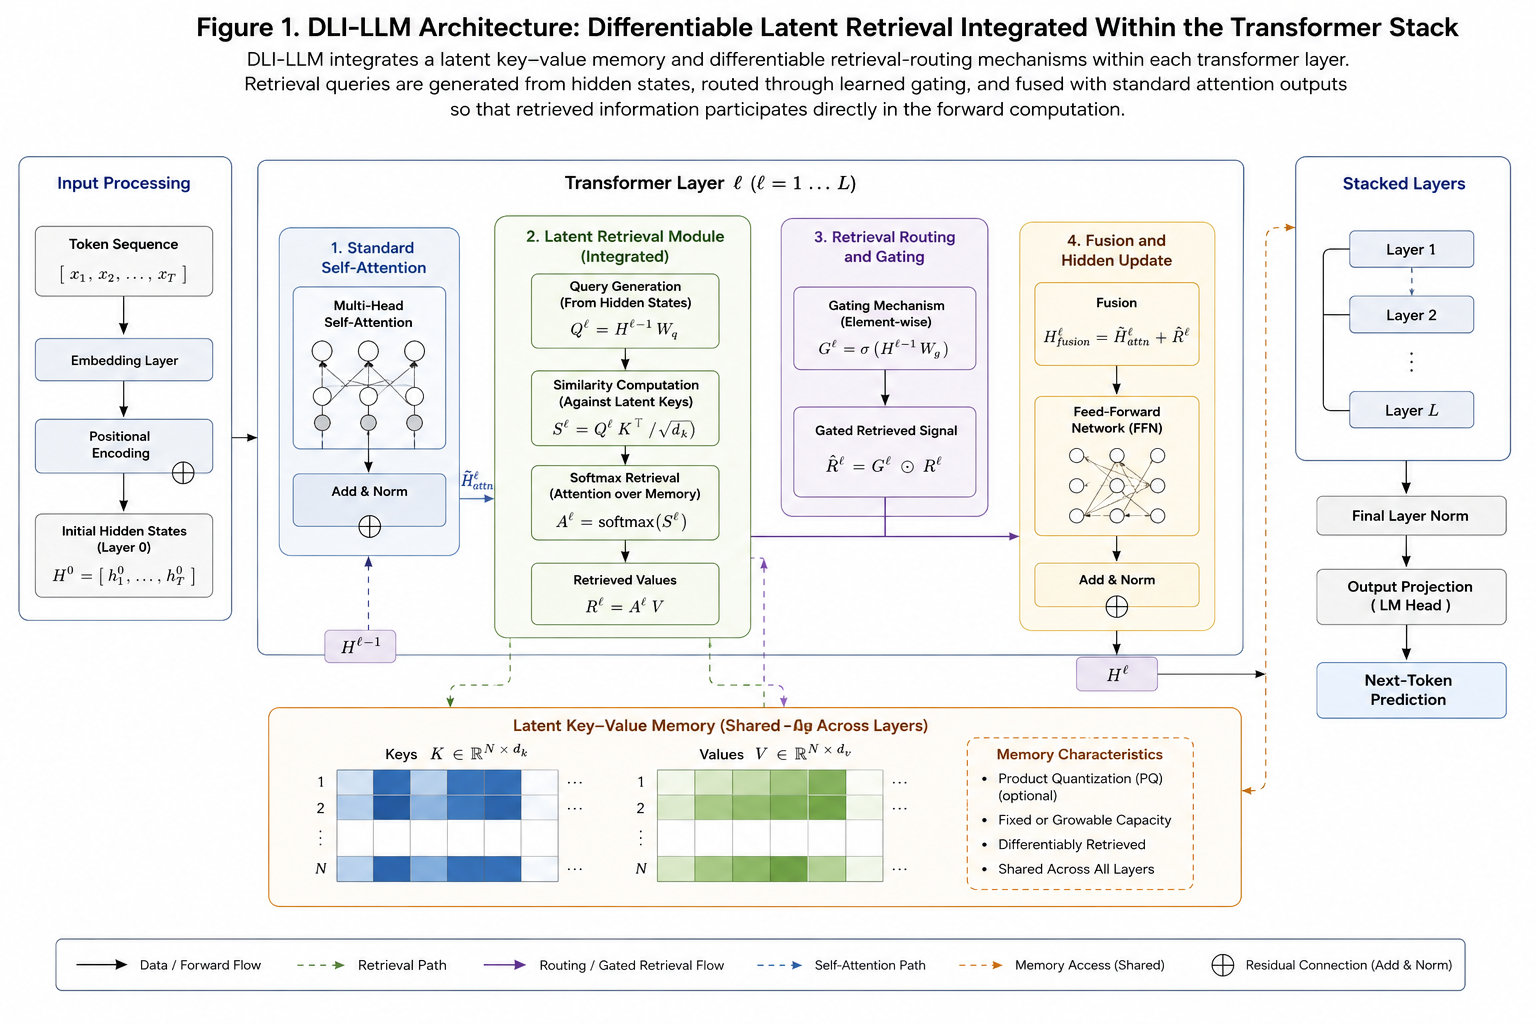
\includegraphics[width=5.49073in,height=3.66383in]{figures/prologue1.png}
\textbf{Figure} 4. Conceptual illustration of retrieval fragmentation and modality separation in conventional retrieval-augmented architectures.
The figure does not present empirical benchmark data and should instead be interpreted as a theoretical comparative model derived from architectural analysis and prior observations in memory-augmented transformer research.
\hypertarget{broader-architectural-implications}{%
\subsection{Broader Architectural Implications}}
\label{broader-architectural-implications}
More broadly, DLI-LLM contributes to ongoing research exploring how retrieval, memory coordination, and contextual inference may become more tightly integrated within transformer-based architectures. Rather than treating retrieval exclusively as an external augmentation layer, the framework proposes a conceptual direction in which latent retrieval mechanisms participate directly in model computation.
Although the present work remains theoretical and requires empirical validation, it provides a formal architectural basis for future investigation into retrieval-integrated transformer architectures and differentiable coordination of latent memory.
\hypertarget{closing}{%
\section{Closing thoughts}}
\label{closing}
This paper formalized the \emph{DLI-LLM hypothesis} as a conceptual architectural framework for integrating differentiable latent retrieval directly within transformer-layer computation. Unlike conventional
retrieval-augmented architectures that maintain an operational separation between retrieval and inference, the proposed framework introduces a unified latent retrieval pathway operating within the transformer\textquotesingle s forward pass.
The work presented a mathematical formulation of differentiable latent retrieval, an implementation-oriented architectural model, and a comparative analysis relative to existing memory-augmented and retrieval-integrated transformer systems. In addition, the paper examined predicted architectural behaviors, retrieval dynamics, and potential limitations associated with latent memory integration.
Although the framework remains theoretical and requires empirical validation, the proposed architecture provides a structured basis for future investigation into retrieval-integrated transformer architectures, differentiable memory coordination, and latent retrieval mechanisms operating directly within the model's computational pathways.
